% -*- mode: latex; mode: flyspell; ispell-local-dictionary: "en_US"; coding: utf-8; fill-column: 80 -*-

\documentclass[landscape]{article}

\usepackage[utf8]{inputenc}
\usepackage[english]{babel}

\usepackage{amsmath,amsfonts,amssymb}
\usepackage{fullpage}
\usepackage{verbatim}

\usepackage[margin=10mm, top=5mm, bottom=5mm]{geometry}

\usepackage{tikz,pgfplots}

\pgfplotsset{
  width=240mm,height=180mm,
  major grid style={thin,dotted,color=black!50},
  minor grid style={thin,dotted,color=black!50},
  grid,
  every axis/.append style={
    line width=0.5pt,
    tick style={
      line cap=round,
      thin,
      major tick length=4pt,
      minor tick length=2pt,
    },
  },
  legend cell align=left,
  legend pos=north west,
  compat=1.9
}

%%%%%%%%%%%%%%%%%%%%%%%%%%%%%%%%%%%%%%%%%%%%%%%%%%%%%%%%%%%%%%%%%%%%%%%%%%%%%%%%

\begin{document}

% IMPORT-DATA Results Results.txt

\begin{center}

\begin{tikzpicture}
  \begin{axis}[
    title={Bcast},
    xlabel={PEs [$\log_2(n)$]},
    ylabel={Run Time},
    ]

    %% MULTIPLOT(Type) SELECT PEs AS x, Time as y, MULTIPLOT FROM (    
    %% SELECT benchmark, LOG(2, size) AS PEs, MEDIAN(time) as Time, 'Median' as Type FROM `Results`
    %% WHERE iteration>0
    %% GROUP BY benchmark, size
    %% UNION ALL
    %% SELECT benchmark, LOG(2, size) AS PEs, MIN(time) as Time, 'Min' as Type FROM `Results`
    %% WHERE iteration>0
    %% GROUP BY benchmark, size
    %% UNION ALL
    %% SELECT benchmark, LOG(2, size) AS PEs, MAX(time) as Time, 'Max' as Type FROM `Results`
    %% WHERE iteration>0
    %% GROUP BY benchmark, size
    %% ) a
    %% WHERE benchmark = 'bcast' AND PEs<11
    %% GROUP BY MULTIPLOT, x  ORDER BY MULTIPLOT, x
    \addplot coordinates { (5.0,0.000212) (6.0,0.000329) (7.0,0.000464) (8.0,0.000629) (9.0,0.000696) (10.0,0.000836001) };
    \addlegendentry{Type=Max};
    \addplot coordinates { (5.0,6.99982e-06) (6.0,1.49999e-05) (7.0,2.10004e-05) (8.0,2.59997e-05) (9.0,3.70005e-05) (10.0,4.39999e-05) };
    \addlegendentry{Type=Median};
    \addplot coordinates { (5.0,5.99958e-06) (6.0,1.10008e-05) (7.0,1.49999e-05) (8.0,1.59992e-05) (9.0,2.50004e-05) (10.0,3.39998e-05) };
    \addlegendentry{Type=Min};

  \end{axis}
\end{tikzpicture}

\newpage
\begin{tikzpicture}
  \begin{axis}[
    title={BcastMPI},
    xlabel={PEs [$\log_2(n)$]},
    ylabel={Run Time},
    ]

    %% MULTIPLOT(Type) SELECT PEs AS x, Time as y, MULTIPLOT FROM ( 
    %% SELECT benchmark, LOG(2, size) AS PEs, MEDIAN(time) as Time, 'Median' as Type FROM `Results`
    %% WHERE iteration>0
    %% GROUP BY benchmark, size
    %% UNION ALL
    %% SELECT benchmark, LOG(2, size) AS PEs, MIN(time) as Time, 'Min' as Type FROM `Results`
    %% WHERE iteration>0
    %% GROUP BY benchmark, size
    %% UNION ALL
    %% SELECT benchmark, LOG(2, size) AS PEs, MAX(time) as Time, 'Max' as Type FROM `Results`
    %% WHERE iteration>0
    %% GROUP BY benchmark, size
    %% ) a
    %% WHERE benchmark = 'bcastMPI' AND PEs<11
    %% GROUP BY MULTIPLOT, x  ORDER BY MULTIPLOT, x
    \addplot coordinates { (5.0,1.09999e-05) (6.0,1.70004e-05) (7.0,2.00002e-05) (8.0,5.29997e-05) (9.0,5.00004e-05) (10.0,4.39999e-05) };
    \addlegendentry{Type=Max};
    \addplot coordinates { (5.0,6.00051e-06) (6.0,9.0003e-06) (7.0,1.20001e-05) (8.0,1.89999e-05) (9.0,2.50004e-05) (10.0,3.29996e-05) };
    \addlegendentry{Type=Median};
    \addplot coordinates { (5.0,5.00027e-06) (6.0,6.00051e-06) (7.0,8.99937e-06) (8.0,8.00006e-06) (9.0,1.89999e-05) (10.0,2.99998e-05) };
    \addlegendentry{Type=Min};

  \end{axis}
\end{tikzpicture}
\newpage

\begin{tikzpicture}
\begin{axis}[
title={BcastReverseMPI},
xlabel={PEs [$\log_2(n)$]},
ylabel={Run Time},
]

%% MULTIPLOT(Type) SELECT PEs AS x, Time as y, MULTIPLOT FROM ( 
%% SELECT benchmark, LOG(2, size) AS PEs, MEDIAN(time) as Time, 'Median' as Type FROM `Results`
%% WHERE iteration>0
%% GROUP BY benchmark, size
%% UNION ALL
%% SELECT benchmark, LOG(2, size) AS PEs, MIN(time) as Time, 'Min' as Type FROM `Results`
%% WHERE iteration>0
%% GROUP BY benchmark, size
%% UNION ALL
%% SELECT benchmark, LOG(2, size) AS PEs, MAX(time) as Time, 'Max' as Type FROM `Results`
%% WHERE iteration>0
%% GROUP BY benchmark, size
%% ) a
%% WHERE benchmark = 'bcastReverseMPI'
%% GROUP BY MULTIPLOT, x  ORDER BY MULTIPLOT, x
\addplot coordinates { (5.0,0.000179) (6.0,0.000306999) (7.0,0.000326999) (8.0,0.000307) (9.0,0.000324) (10.0,0.000351001) (11.0,0.000325999) };
\addlegendentry{Type=Max};
\addplot coordinates { (5.0,1.49999e-05) (6.0,2.20006e-05) (7.0,3.20002e-05) (8.0,4.69992e-05) (9.0,5.39999e-05) (10.0,6.70003e-05) (11.0,8.20002e-05) };
\addlegendentry{Type=Median};
\addplot coordinates { (5.0,1.09999e-05) (6.0,1.40006e-05) (7.0,2.7e-05) (8.0,3.39998e-05) (9.0,4.39994e-05) (10.0,5.20004e-05) (11.0,6.2e-05) };
\addlegendentry{Type=Min};

\end{axis}
\end{tikzpicture}
\newpage
\newpage
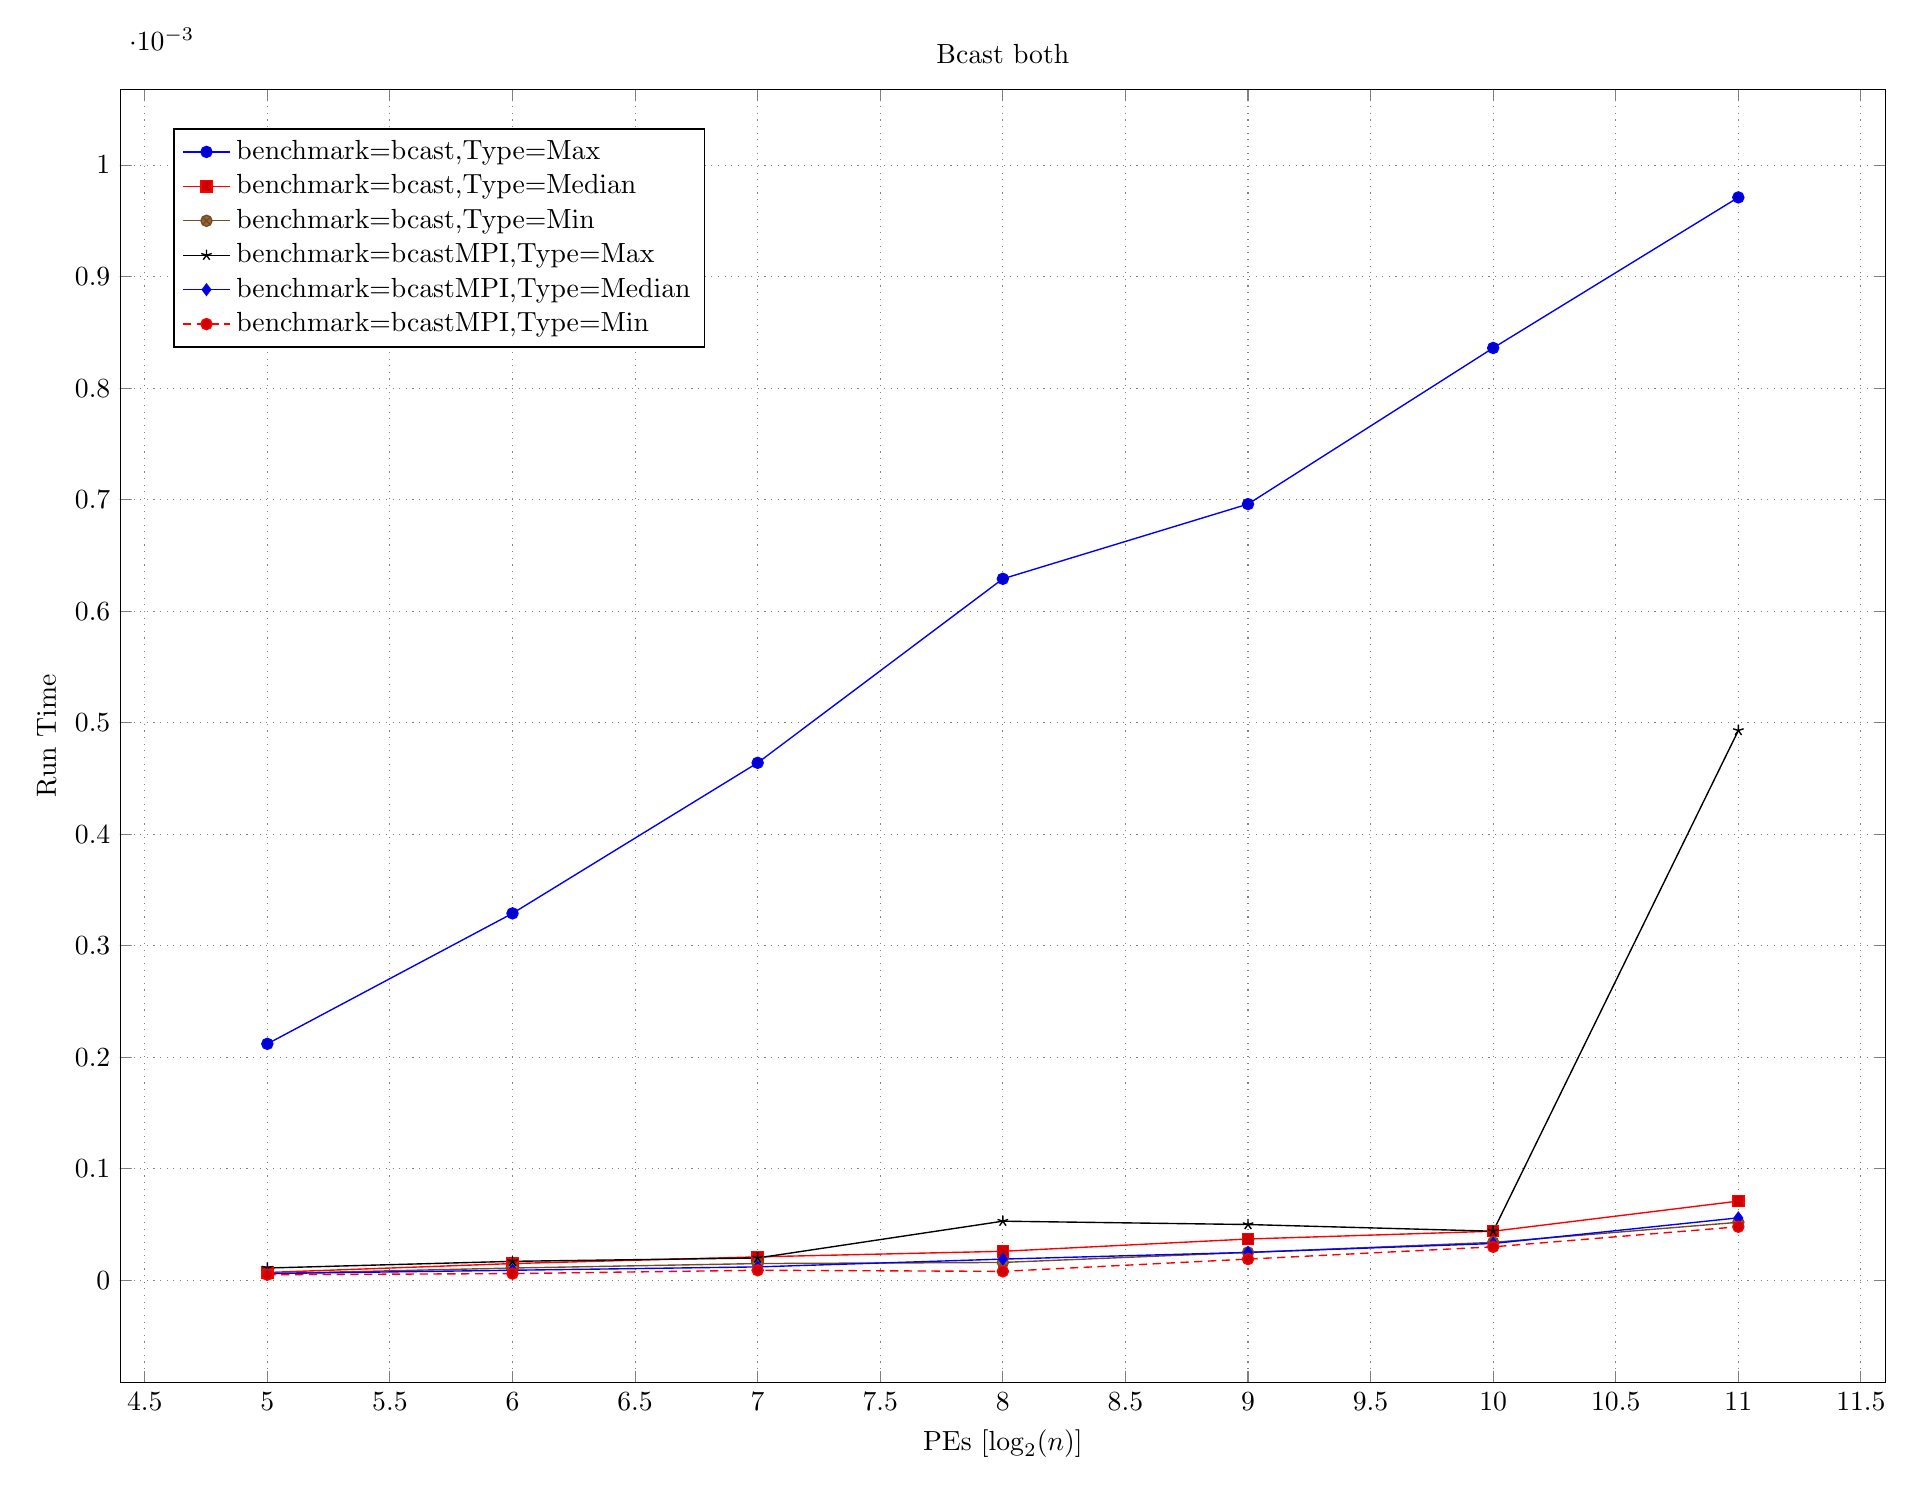
\begin{tikzpicture}
  \begin{axis}[
    title={Bcast both},
    xlabel={PEs [$\log_2(n)$]},
    ylabel={Run Time},
    ]

    %% MULTIPLOT(benchmark, Type) SELECT PEs AS x, Time as y, MULTIPLOT FROM ( 
    %% SELECT benchmark, LOG(2, size) AS PEs, MEDIAN(time) as Time, 'Median' as Type FROM `Results`
    %% WHERE iteration>0
    %% GROUP BY benchmark, size
    %% UNION ALL
    %% SELECT benchmark, LOG(2, size) AS PEs, MIN(time) as Time, 'Min' as Type FROM `Results`
    %% WHERE iteration>0
    %% GROUP BY benchmark, size
    %% UNION ALL
    %% SELECT benchmark, LOG(2, size) AS PEs, MAX(time) as Time, 'Max' as Type FROM `Results`
    %% WHERE iteration>0
    %% GROUP BY benchmark, size
    %% ) a
    %% WHERE benchmark = 'bcast' OR benchmark = 'bcastMPI'
    %% GROUP BY MULTIPLOT, x  ORDER BY MULTIPLOT, x
    \addplot coordinates { (5.0,0.000212) (6.0,0.000329) (7.0,0.000464) (8.0,0.000629) (9.0,0.000696) (10.0,0.000836001) (11.0,0.000971) };
    \addlegendentry{benchmark=bcast,Type=Max};
    \addplot coordinates { (5.0,6.99982e-06) (6.0,1.49999e-05) (7.0,2.10004e-05) (8.0,2.59997e-05) (9.0,3.70005e-05) (10.0,4.39999e-05) (11.0,7.10003e-05) };
    \addlegendentry{benchmark=bcast,Type=Median};
    \addplot coordinates { (5.0,5.99958e-06) (6.0,1.10008e-05) (7.0,1.49999e-05) (8.0,1.59992e-05) (9.0,2.50004e-05) (10.0,3.39998e-05) (11.0,5.19995e-05) };
    \addlegendentry{benchmark=bcast,Type=Min};
    \addplot coordinates { (5.0,1.09999e-05) (6.0,1.70004e-05) (7.0,2.00002e-05) (8.0,5.29997e-05) (9.0,5.00004e-05) (10.0,4.39999e-05) (11.0,0.000493) };
    \addlegendentry{benchmark=bcastMPI,Type=Max};
    \addplot coordinates { (5.0,6.00051e-06) (6.0,9.0003e-06) (7.0,1.20001e-05) (8.0,1.89999e-05) (9.0,2.50004e-05) (10.0,3.29996e-05) (11.0,5.59995e-05) };
    \addlegendentry{benchmark=bcastMPI,Type=Median};
    \addplot coordinates { (5.0,5.00027e-06) (6.0,6.00051e-06) (7.0,8.99937e-06) (8.0,8.00006e-06) (9.0,1.89999e-05) (10.0,2.99998e-05) (11.0,4.79994e-05) };
    \addlegendentry{benchmark=bcastMPI,Type=Min};

  \end{axis}
\end{tikzpicture}

\newpage
\begin{tikzpicture}
  \begin{axis}[
    title={ScanAndBcast},
    xlabel={PEs [$\log_2(n)$]},
    ylabel={Run Time},
    ]

    %% MULTIPLOT(Type) SELECT PEs AS x, Time as y, MULTIPLOT FROM ( 
    %% SELECT benchmark, LOG(2, size) AS PEs, MEDIAN(time) as Time, 'Median' as Type FROM `Results`
    %% WHERE iteration>0
    %% GROUP BY benchmark, size
    %% UNION ALL
    %% SELECT benchmark, LOG(2, size) AS PEs, MIN(time) as Time, 'Min' as Type FROM `Results`
    %% WHERE iteration>0
    %% GROUP BY benchmark, size
    %% UNION ALL
    %% SELECT benchmark, LOG(2, size) AS PEs, MAX(time) as Time, 'Max' as Type FROM `Results`
    %% WHERE iteration>0
    %% GROUP BY benchmark, size
    %% ) a
    %% WHERE benchmark = 'scanAndBcast'
    %% GROUP BY MULTIPLOT, x  ORDER BY MULTIPLOT, x
    \addplot coordinates { (5.0,2.40002e-05) (6.0,3.5e-05) (7.0,6.40005e-05) (8.0,7.29999e-05) (9.0,0.000346) (10.0,0.000267) (11.0,0.000123) };
    \addlegendentry{Type=Max};
    \addplot coordinates { (5.0,2.19997e-05) (6.0,2.29999e-05) (7.0,3.5e-05) (8.0,4.10005e-05) (9.0,6.40005e-05) (10.0,6.30002e-05) (11.0,8.59993e-05) };
    \addlegendentry{Type=Median};
    \addplot coordinates { (5.0,2.00002e-05) (6.0,1.89999e-05) (7.0,3.1e-05) (8.0,3.80008e-05) (9.0,4.99999e-05) (10.0,5.69997e-05) (11.0,7.69999e-05) };
    \addlegendentry{Type=Min};

  \end{axis}
\end{tikzpicture}
\newpage

\newpage
\begin{tikzpicture}
  \begin{axis}[
    title={ScanAndBcastMPI},
    xlabel={PEs [$\log_2(n)$]},
    ylabel={Run Time},
    ]

    %% MULTIPLOT(Type) SELECT PEs AS x, Time as y, MULTIPLOT FROM ( 
    %% SELECT benchmark, LOG(2, size) AS PEs, MEDIAN(time) as Time, 'Median' as Type FROM `Results`
    %% WHERE iteration>0
    %% GROUP BY benchmark, size
    %% UNION ALL
    %% SELECT benchmark, LOG(2, size) AS PEs, MIN(time) as Time, 'Min' as Type FROM `Results`
    %% WHERE iteration>0
    %% GROUP BY benchmark, size
    %% UNION ALL
    %% SELECT benchmark, LOG(2, size) AS PEs, MAX(time) as Time, 'Max' as Type FROM `Results`
    %% WHERE iteration>0
    %% GROUP BY benchmark, size
    %% ) a
    %% WHERE benchmark = 'scanAndBcastMPI'
    %% GROUP BY MULTIPLOT, x  ORDER BY MULTIPLOT, x
    \addplot coordinates { (5.0,6.39996e-05) (6.0,0.000119001) (7.0,0.000235) (8.0,0.000403) (9.0,0.000987001) (10.0,0.001773) (11.0,0.003875) };
    \addlegendentry{Type=Max};
    \addplot coordinates { (5.0,3.80008e-05) (6.0,7.20005e-05) (7.0,0.000144) (8.0,0.000252) (9.0,0.000603) (10.0,0.001048) (11.0,0.002289) };
    \addlegendentry{Type=Median};
    \addplot coordinates { (5.0,3.5e-05) (6.0,6.69993e-05) (7.0,0.000134001) (8.0,0.000242) (9.0,0.000487) (10.0,0.000978) (11.0,0.002127) };
    \addlegendentry{Type=Min};

  \end{axis}
\end{tikzpicture}

\newpage
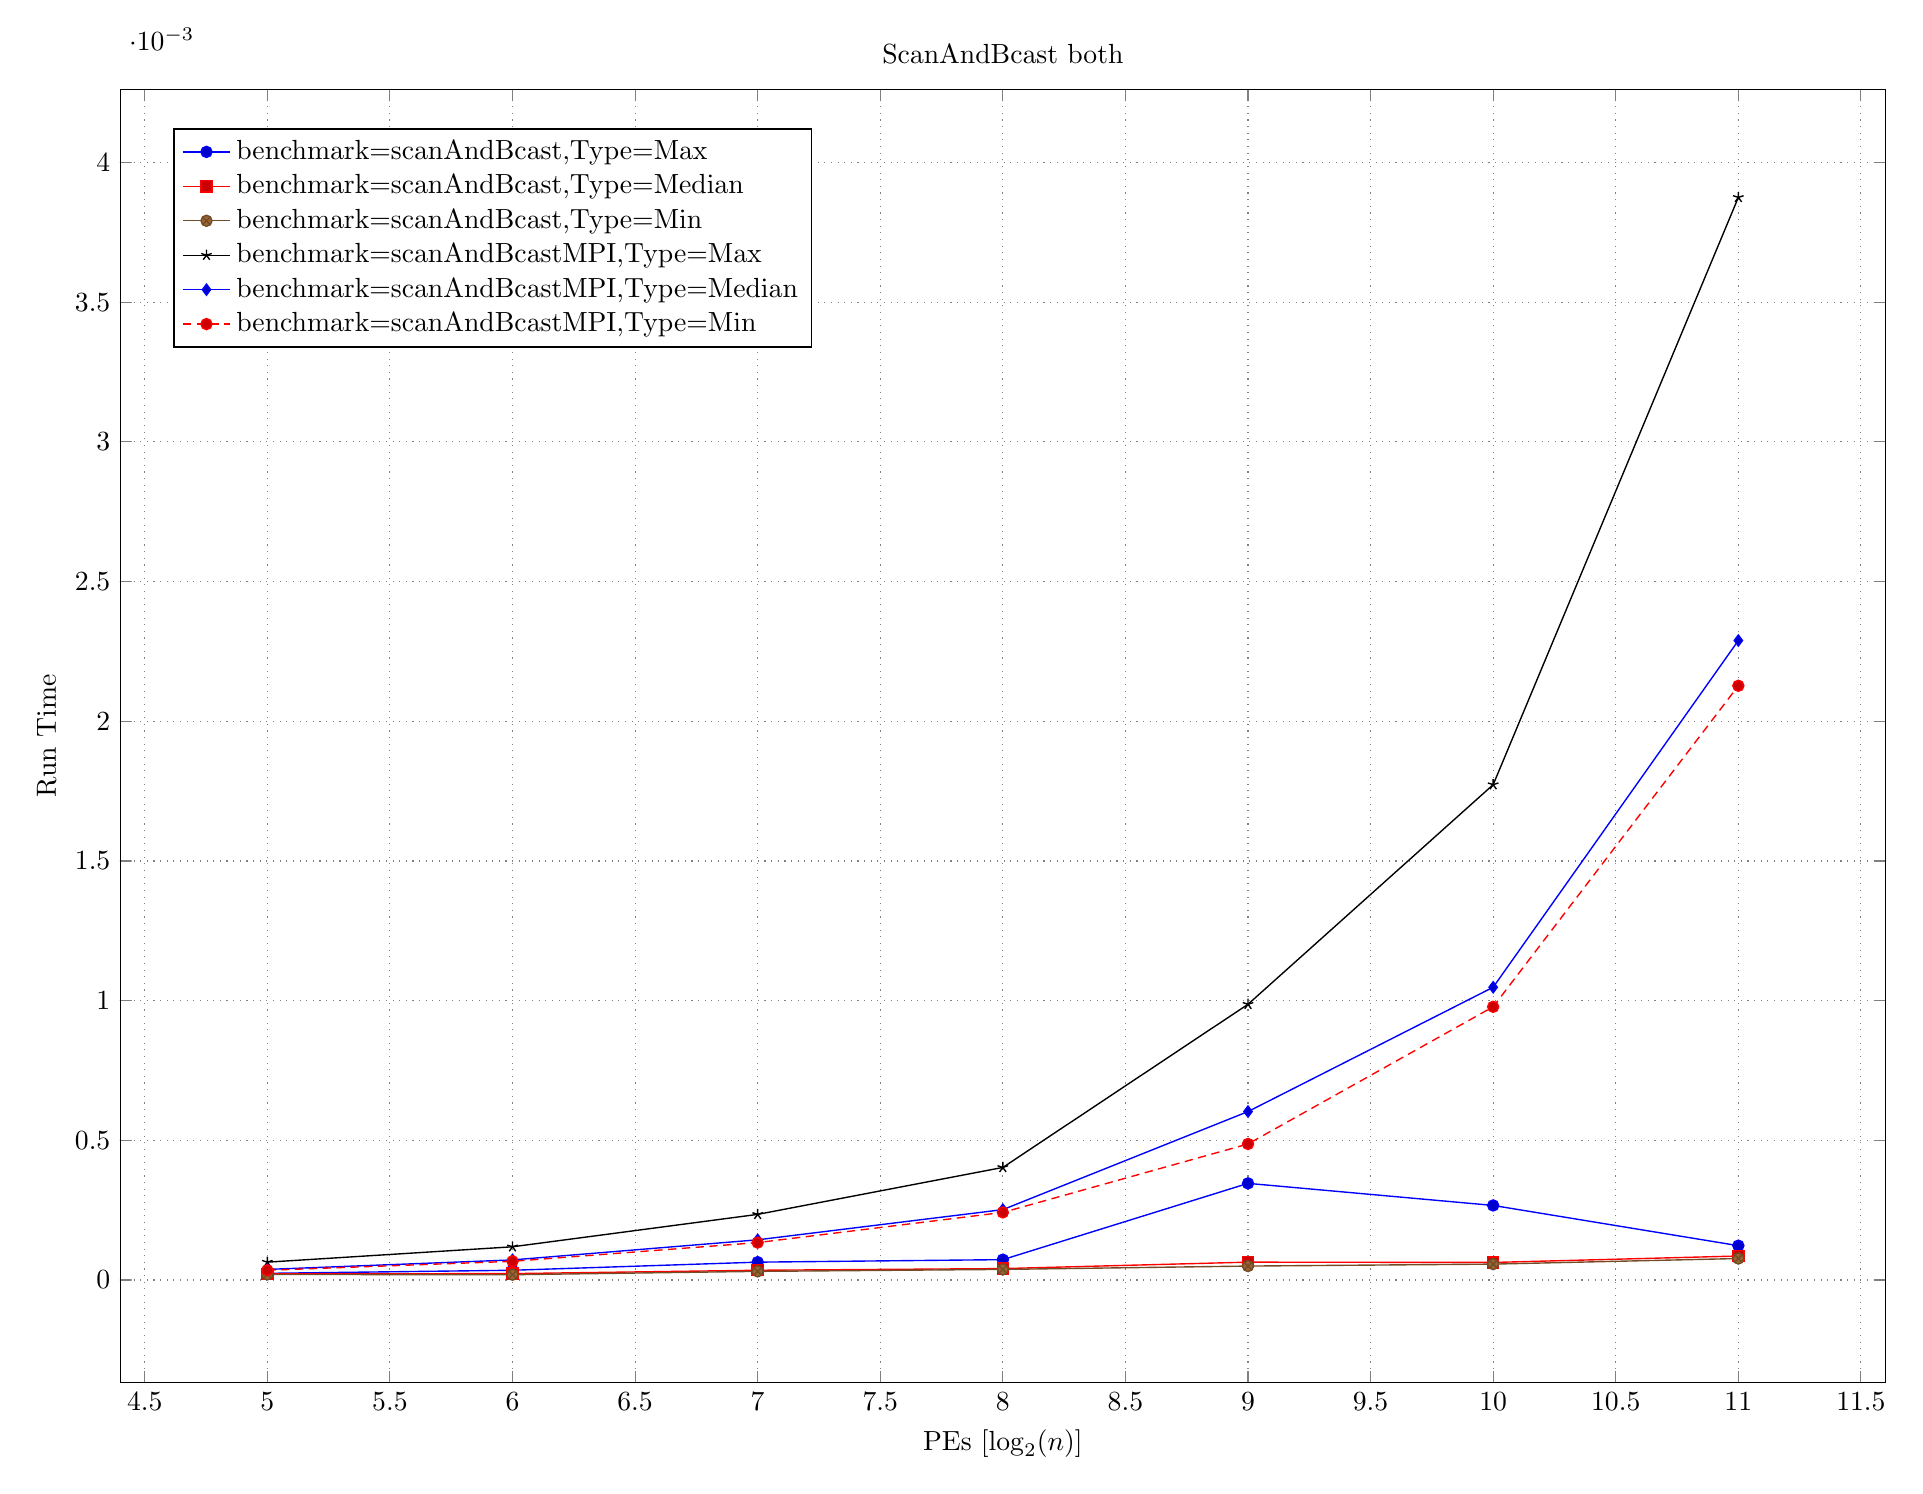
\begin{tikzpicture}
  \begin{axis}[
    title={ScanAndBcast both},
    xlabel={PEs [$\log_2(n)$]},
    ylabel={Run Time},
    ]

    %% MULTIPLOT(benchmark, Type) SELECT PEs AS x, Time as y, MULTIPLOT FROM ( 
    %% SELECT benchmark, LOG(2, size) AS PEs, MEDIAN(time) as Time, 'Median' as Type FROM `Results`
    %% WHERE iteration>0
    %% GROUP BY benchmark, size
    %% UNION ALL
    %% SELECT benchmark, LOG(2, size) AS PEs, MIN(time) as Time, 'Min' as Type FROM `Results`
    %% WHERE iteration>0
    %% GROUP BY benchmark, size
    %% UNION ALL
    %% SELECT benchmark, LOG(2, size) AS PEs, MAX(time) as Time, 'Max' as Type FROM `Results`
    %% WHERE iteration>0
    %% GROUP BY benchmark, size
    %% ) a
    %% WHERE benchmark = 'scanAndBcast' OR benchmark = 'scanAndBcastMPI'
    %% GROUP BY MULTIPLOT, x  ORDER BY MULTIPLOT, x
    \addplot coordinates { (5.0,2.40002e-05) (6.0,3.5e-05) (7.0,6.40005e-05) (8.0,7.29999e-05) (9.0,0.000346) (10.0,0.000267) (11.0,0.000123) };
    \addlegendentry{benchmark=scanAndBcast,Type=Max};
    \addplot coordinates { (5.0,2.19997e-05) (6.0,2.29999e-05) (7.0,3.5e-05) (8.0,4.10005e-05) (9.0,6.40005e-05) (10.0,6.30002e-05) (11.0,8.59993e-05) };
    \addlegendentry{benchmark=scanAndBcast,Type=Median};
    \addplot coordinates { (5.0,2.00002e-05) (6.0,1.89999e-05) (7.0,3.1e-05) (8.0,3.80008e-05) (9.0,4.99999e-05) (10.0,5.69997e-05) (11.0,7.69999e-05) };
    \addlegendentry{benchmark=scanAndBcast,Type=Min};
    \addplot coordinates { (5.0,6.39996e-05) (6.0,0.000119001) (7.0,0.000235) (8.0,0.000403) (9.0,0.000987001) (10.0,0.001773) (11.0,0.003875) };
    \addlegendentry{benchmark=scanAndBcastMPI,Type=Max};
    \addplot coordinates { (5.0,3.80008e-05) (6.0,7.20005e-05) (7.0,0.000144) (8.0,0.000252) (9.0,0.000603) (10.0,0.001048) (11.0,0.002289) };
    \addlegendentry{benchmark=scanAndBcastMPI,Type=Median};
    \addplot coordinates { (5.0,3.5e-05) (6.0,6.69993e-05) (7.0,0.000134001) (8.0,0.000242) (9.0,0.000487) (10.0,0.000978) (11.0,0.002127) };
    \addlegendentry{benchmark=scanAndBcastMPI,Type=Min};

  \end{axis}
\end{tikzpicture}
\newpage


\newpage
\begin{tikzpicture}
\begin{axis}[
title={SplitCommOnce},
xlabel={PEs [$\log_2(n)$]},
ylabel={Run Time},
]

%% MULTIPLOT(Type) SELECT PEs AS x, Time as y, MULTIPLOT FROM ( 
%% SELECT benchmark, LOG(2, size) AS PEs, MEDIAN(time) as Time, 'Median' as Type FROM `Results`
%% WHERE iteration>0
%% GROUP BY benchmark, size
%% UNION ALL
%% SELECT benchmark, LOG(2, size) AS PEs, MIN(time) as Time, 'Min' as Type FROM `Results`
%% WHERE iteration>0
%% GROUP BY benchmark, size
%% UNION ALL
%% SELECT benchmark, LOG(2, size) AS PEs, MAX(time) as Time, 'Max' as Type FROM `Results`
%% WHERE iteration>0
%% GROUP BY benchmark, size
%% ) a
%% WHERE benchmark = 'splitCommOnce'
%% GROUP BY MULTIPLOT, x  ORDER BY MULTIPLOT, x
\addplot coordinates { (5.0,8.70004e-05) (6.0,0.000335) (7.0,0.000318) (8.0,0.00038) (9.0,0.00158) (10.0,0.000721999) (11.0,0.00098) };
\addlegendentry{Type=Max};
\addplot coordinates { (5.0,6.09998e-05) (6.0,7.60006e-05) (7.0,0.000185001) (8.0,0.000269) (9.0,0.000423) (10.0,0.000522) (11.0,0.000763) };
\addlegendentry{Type=Median};
\addplot coordinates { (5.0,5.69997e-05) (6.0,7.20005e-05) (7.0,0.000174001) (8.0,0.000253) (9.0,0.000406) (10.0,0.000481) (11.0,0.000718) };
\addlegendentry{Type=Min};

\end{axis}
\end{tikzpicture}

\newpage
\begin{tikzpicture}
\begin{axis}[
title={SplitCommOnce\_split},
xlabel={PEs [$\log_2(n)$]},
ylabel={Run Time},
]

%% MULTIPLOT(Type) SELECT PEs AS x, Time as y, MULTIPLOT FROM ( 
%% SELECT benchmark, LOG(2, size) AS PEs, MEDIAN(time) as Time, 'Median' as Type FROM `Results`
%% WHERE iteration>0
%% GROUP BY benchmark, size
%% UNION ALL
%% SELECT benchmark, LOG(2, size) AS PEs, MIN(time) as Time, 'Min' as Type FROM `Results`
%% WHERE iteration>0
%% GROUP BY benchmark, size
%% UNION ALL
%% SELECT benchmark, LOG(2, size) AS PEs, MAX(time) as Time, 'Max' as Type FROM `Results`
%% WHERE iteration>0
%% GROUP BY benchmark, size
%% ) a
%% WHERE benchmark = 'splitCommOnce_split'
%% GROUP BY MULTIPLOT, x  ORDER BY MULTIPLOT, x
\addplot coordinates { (5.0,9.10005e-05) (6.0,0.000381) (7.0,0.000747) (8.0,0.001095) (9.0,0.001035) (10.0,0.000864) (11.0,0.001424) };
\addlegendentry{Type=Max};
\addplot coordinates { (5.0,7.60006e-05) (6.0,0.000137) (7.0,0.000271) (8.0,0.000407) (9.0,0.000617) (10.0,0.000832001) (11.0,0.001252) };
\addlegendentry{Type=Median};
\addplot coordinates { (5.0,7.10003e-05) (6.0,0.000128) (7.0,0.000254001) (8.0,0.000386001) (9.0,0.000593999) (10.0,0.000807) (11.0,0.001222) };
\addlegendentry{Type=Min};

\end{axis}
\end{tikzpicture}

\newpage
\begin{tikzpicture}
\begin{axis}[
title={SplitCommRecursive},
xlabel={PEs [$\log_2(n)$]},
ylabel={Run Time},
]

%% MULTIPLOT(Type) SELECT PEs AS x, Time as y, MULTIPLOT FROM ( 
%% SELECT benchmark, LOG(2, size) AS PEs, MEDIAN(time) as Time, 'Median' as Type FROM `Results`
%% WHERE iteration>0
%% GROUP BY benchmark, size
%% UNION ALL
%% SELECT benchmark, LOG(2, size) AS PEs, MIN(time) as Time, 'Min' as Type FROM `Results`
%% WHERE iteration>0
%% GROUP BY benchmark, size
%% UNION ALL
%% SELECT benchmark, LOG(2, size) AS PEs, MAX(time) as Time, 'Max' as Type FROM `Results`
%% WHERE iteration>0
%% GROUP BY benchmark, size
%% ) a
%% WHERE benchmark = 'splitCommRecursive'
%% GROUP BY MULTIPLOT, x  ORDER BY MULTIPLOT, x
\addplot coordinates { (5.0,0.001093) (6.0,0.002433) (7.0,0.004348) (8.0,0.009134) (9.0,0.019148) (10.0,0.037085) (11.0,0.07766) };
\addlegendentry{Type=Max};
\addplot coordinates { (5.0,0.000829999) (6.0,0.001865) (7.0,0.003551) (8.0,0.007651) (9.0,0.016128) (10.0,0.033624) (11.0,0.072863) };
\addlegendentry{Type=Median};
\addplot coordinates { (5.0,0.000815) (6.0,0.001804) (7.0,0.003503) (8.0,0.007569) (9.0,0.016015) (10.0,0.033368) (11.0,0.071966) };
\addlegendentry{Type=Min};

\end{axis}
\end{tikzpicture}

\end{center}

\end{document}

%%%%%%%%%%%%%%%%%%%%%%%%%%%%%%%%%%%%%%%%%%%%%%%%%%%%%%%%%%%%%%%%%%%%%%%%%%%%%%%%
